
%(BEGIN_QUESTION)
% Copyright 2006, Tony R. Kuphaldt, released under the Creative Commons Attribution License (v 1.0)
% This means you may do almost anything with this work of mine, so long as you give me proper credit

Graph the response of a proportional+derivative controller to the following input conditions, assuming a proportional band of 200\% and a derivative constant of 15 seconds.  The controller's action is {\it reverse}, and the algorithm it follows is shown below the graph:

$$\includegraphics[width=15.5cm]{i01546x01.eps}$$

The time scale on the chart is minutes:seconds, and the P+D algorithm is as follows:

$$m = K_p \left( e + \tau_d {de \over dt} \right) + b$$

\noindent
Where,

$m$ = Controller output (manipulated variable)

$K_p$ = Gain

$e$ = Error signal (SP$-$PV)

$\tau_d$ = Derivative time constant

$b$ = Bias

\vskip 10pt

\underbar{file i01546}
%(END_QUESTION)





%(BEGIN_ANSWER)

%$$\includegraphics[width=15.5cm]{i01546x02.eps}$$
$$\includegraphics[width=15.5cm]{i01546x03.eps}$$

When the PV begins its initial upward ramp from 35\% to 60\%, it does so at a slope of 100\% per minute (25\% over a 15 second period of time).  Since derivative action is the slope multiplied by the derivative constant (15 seconds, or 1/4 minute), multiplied by the gain (PB of 200\% = gain of 0.5), the derivative term's action here is to step down 12.5\%.  Then, we see proportional action (with a gain of 0.5) ramp the output down at a slope 1/2 that of the PV's slope, to a point of 55\%.  

Then, when the PV ramp reverses direction and descends at the same rate it ascended previously, the derivative action stops {\it subtracting} 12.5\% from the output and begins to {\it add} 12.5\% to the output, for a total step-change in the output of 25\% (from 55\% to 80\%).  Proportional action, of course, ramps the output up 12.5\% from time 0:45 to time 1:00 (from 80\% to 92.5\%) as the PV changes 25\% in 15 seconds.  When the PV levels off at 1:00, at the same value it stated at, the derivative action ceases, and the output returns to its original value of 80\%.

At time 1:15, the 15\% downward step-change taken by the PV causes derivative action to go ``wild'' and saturate the output at 100\%.  Proportional action steps up the output by 7.5\%, so that after the transient rise of the PV the output settles at 87.5\%.  At time 1:45, the 15\% upward step-change of the PV causes derivative action to saturate the output once more, this time in the downward direction at 0\%.  After this transient, the output settles at 75\%: a combined effect of proportional action (driving the output down to 80\%) and derivative action (driving the output down 5\%, because the PV's upward slope is 40\% per minute -- 40\%/min times 0.25 minutes times a $K_p$ of 0.5).  Proportional action ramps the output down 10\% (from 75\% to 65\%) until time 2:15, when the ramping stops and derivative action ceases, allowing the output to step up by 5\% (from 65\% to 70\%) to its final value.

%(END_ANSWER)





%(BEGIN_NOTES)


%INDEX% Control, proportional + derivative: graphing controller response

%(END_NOTES)


